%
% lambertw.tex
%
% (c) 2021 Prof Dr Andreas Müller, OST Ostschweizer Fachhochschule
%
\section{Die Lambert $W$-Funktion
\label{buch:section:lambertw}}
\rhead{Lambert $W$-Funktion}
Exponentialgleichungen wie
\[
e^{2x}+2e^x-15=0
\]
können durch Substitution $y=e^x$ in eine algebraische Gleichung
umgeformt werden, die mit Wurzelfunktionen gelöst werden kann.
Eine solche Substitution ist nicht mehr möglich, wenn Produkte
der Unbekannten und der Exponentialfunktion, also $xe^x$ auftreten.
Die Lambert $W$-Funktion ermöglicht, die Lösungen solcher Gleichungen
darzustellen.

Als Anwendung der Theorie der Lambert-$W$-Funktion wird in
Kapitel~\ref{chapter:lambertw}
eine Parametrisierung einer Verfolgungskurve mit Hilfe von $W(x)$
bestimmt.

%
% Die Funktion xe^x
%
\subsection{Die Definition der Lambert $W$-Funktion
\label{buch:subsection:funktion-xexpx}}
\begin{figure}
\centering
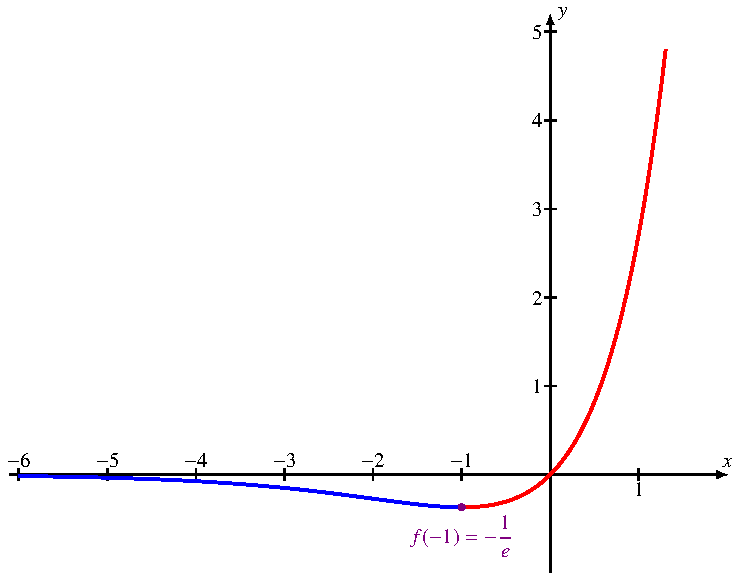
\includegraphics{chapters/020-exponential/images/xexpx.pdf}
\caption{Graph der Funktion $f\colon x\mapsto f(x)=xe^x$
\label{buch:lambert:graph}}
\end{figure}
Ein Graph der Funktion 
\[
f\colon \mathbb{R}\to\mathbb{R} : x\mapsto xe^x
\]
ist in Abbildung~\ref{buch:lambert:graph} dargestellt.
Die einzige Nullstelle ist bei $x=0$.
Die Funktion $f$ hat die Ableitung
$f'(x)=e^x + xe^x$,
an  der Stelle $x=0$ hat der Graph von $f(x)$ daher die Steigung $1$.

Die Ableitung verschwindet für
\[
0 = f'(x) = e^x(1+x)
\qquad\Rightarrow\qquad
x=-1,
\]
dort hat die Funktion $f$ den minimalen Wert $-1/e$.

Wegen des Minimums an der Stelle $x=-1$ ist die Funktion $f(x)$ nicht
umkehrbar.
Auf dem Teilintervall $I_{-1}=(-\infty,-1]$ ist $f$ streng
monoton fallend, auf dem Teilintervall $I_0=[-1,\infty)$ ist sie
streng monoton wachsen.
Die Einschränkung von $f$ auf diese beiden Intervalle ist also
invertierbar.

\begin{definition}
Die inverse Funktion der Funktion $[-1,\infty)\to[-1/e,\infty):x\mapsto xe^x=y$
heisst die Lambert $W$-Funktion, geschrieben $W(y)$ oder $W_0(y)$.
\index{Lambert-W-Funktion@Lambert-$W$-Funktion!Definition}%
Die inverse Funktion der Funktion $(-\infty,-1)\to[-1/e,0)$ wird mit
$W_{-1}$ bezeichnet.
\index{Lambert-W-Funktion@Lambert-$W$-Funktion!Graph}%
\end{definition}

\begin{figure}
\centering
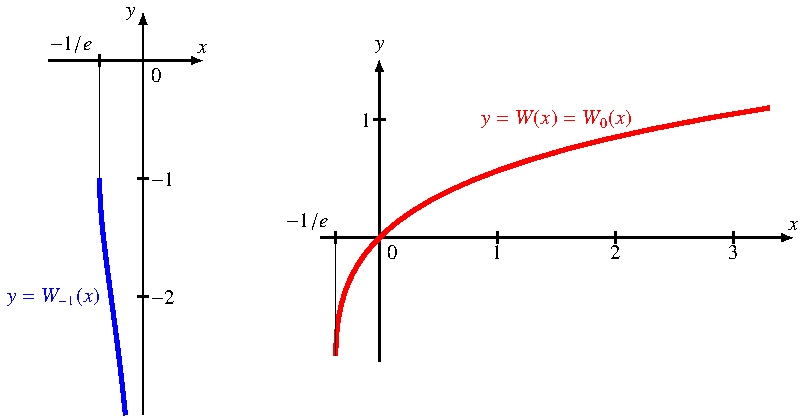
\includegraphics{chapters/020-exponential/images/w.pdf}
\caption{Graph der Funktionen $W_{-1}(x)$ (links) und $W_0(x)$ (rechts)
\label{buch:lambert:wgraph}}
\end{figure}
Die beiden Funktion $W_0(x)$ und $W_{-1}(x)$ sind in
Abbildung~\ref{buch:lambert:wgraph} dargestellt.
Beide Funktionen sind streng monoton und haben unendlich grosse Steigung
an der Stelle $x=-1/e$.

Da die $W$-Funktionen Umkehrfunktionen der Funktion $f(x)=xe^x$ sind,
erfüllen sie
\[
W(x) e^{W(x)} = x.
\]

%
% Ableitung der W-Funktion
%
\subsubsection{Ableitung der Funktionen $W(x)$ und $W_{-1}(x)$}
\index{Lambert-W-Funktion@Lambert-$W$-Funktion!Ableitung}
Die Umkehrfunktion $f^{-1}(y)$ einer Funktion $f(x)$ erfüllt
\(
f^{-1}(f(x)) = x.
\)
Ableitung nach $x$ ergibt mit der Kettenregel
\[
\frac{df^{-1}(y)}{dy}\bigg|_{y=f(x)} \frac{df}{dx} = 0
\qquad\Rightarrow\qquad
(f^{-1})'(y) = \frac{1}{f'(x)}.
\]
Für die $W$-Funktion, also für $W(y)=x$ oder $y=f(x)=xe^x$ bedeutet dies
\[
W'(y)
=
\frac{1}{f'(x)}
=
\frac{1}{f'(W(y))}.
\]
Die Ableitung von $f$ an der Stelle $W(y)$ ist
\[
f'(W(y))
=
(1+x)e^x
=
(1+W(y))e^{W(y)}.
\]
Die Exponentialfunktion von $W(y)$ ist
\[
e^{W(y)} = \frac{y}{W(y)},
\]
womit die Ableitung der $W$-Funktion
\begin{equation}
W'(y)
=
\frac{W(y)}{y}\cdot \frac{1}{1+W(y)}
=
\frac{W(y)}{y(1+W(y))}
\label{buch:lambert:eqn:ableitung}
\end{equation}
wird.

Aus der ersten Ableitung kann jetzt mit Hilfe der Quotientenregel
auch jede höhere Ableitung berechnet werden.
Die zweite Ableitung ist
\begin{align*}
\frac{d^2}{dy^2}W(y)
&=
\frac{d}{dy}W'(y)
=
\frac{d}{dy}\frac{W(y)}{y(1+W(y))}
\\
&=
\frac{
W'(y)y(1+W(y)) - W(y)\bigl(1+W(y)+yW'(y)\bigr)
}{
y^2(1+W(y))^2
}
\\
&=
\frac{
W'(y)y - W(y)(1+W(y))
}{
y^2(1+W(y))^2
}.
\intertext{Die Ableitung $W'(y)$ kann jetzt durch
\eqref{buch:lambert:eqn:ableitung} ersetzt werden, dies ergibt}
&=
\frac{
\displaystyle
\frac{W(y)}{y(1+W(y))}y - W(y)(1+W(y))
}{
y^2(1+W(y))^2
}
\\
&=
\frac{
W(y) - W(y)(1+W(y))^2
}{
y^2(1+W(y))^3
}
\\
&=
\frac{
-2W(y)^2-W(y)^3
}{
y^2(1+W(y))^3
}
\\
&=
-
\frac{
W(y)^2
}{
y^2(1+W(y))^3
}
(W(y)+2).
\end{align*}
Nach dem selben Muster können beliebig hohe Ableitungen von $W(y)$ durch
$W(y)$ ausgedrückt werden.
Zum Beispiel findet man nach einiger Rechnung für die dritte und vierte
Ableitung der $W$-Funktion die Ausdrücke
\begin{align*}
W'''(x)
&=
\phantom{-}
\frac{W(y)^3}{y^3(1+W(y))^4}\cdot (2W(y)^2 + 8W(y)+9)
\\
W''''(x)
&=
-\frac{W(y)^4}{y^4(1+W(y))^5}\cdot (6W(y)^3 + 36W(y)^2 + 79W(y) + 64).
\end{align*}
Mit etwas zusätzlicher Arbeit kann man für die $n$-te Ableitung
\[
\frac{d^n}{dy^n} W(y)
=
\frac{(-1)^{n+1}W(y)^n}{y^n(1+W(y))^{n+1}} \cdot P_n(W(y)),
\]
wobei die Polynome $P_n(t)$ die Rekursionsgleichung
\[
P_{n+1}(t)
=
(nt+3n-1)\cdot P_n(t) - (t+1)\cdot P'_n(t)
\]
mit $P_1(t)=1$.

%
% Differentialgleichung und Stammfunktion
%
\subsubsection{Differentialgleichung und Stammfunktion}
\index{Lambert-W-Funktion@Lambert-$W$-Funktion!Differentialgleichung}%
\index{Differentialgleichung!der Lambert-$W$-Funktion}%
Die Ableitungsformel \eqref{buch:lambert:eqn:ableitung} bedeutet auch,
dass die $W$-Funktion eine Lösung der Differentialgleichung
\[
\frac{dW}{dz}
=
\frac{W}{z(1+W)}
\qquad
\text{mit Anfangsbedingung}
\qquad
W(0) = 1
\]
ist.
Diese Gleichung kann separiert werden in
\[
(1+W)\frac{dW}{W} = \frac{dz}{z}.
\]

Eine Stammfunktion
\index{Lambert-W-Funktion@Lambert-$W$-Funktion!Stammfunktion}%
\[
F(y)
=
\int W(y)\,dy
\]
von $W$ kann mit der Substition $w=W(y)$ gefunden
werden, also $we^w=y$.
Die Ableitung ist $dy = (1+w)e^w\,dw$, so dass die Stammfunktion
\begin{align*}
\int W(y)\,dy
&=
\int w (1+w)e^w\,dw
=
(w^2-w+1)e^w+C
\end{align*}
wird.
Durch Rücksubstitution und mit Hilfe der Relation $e^{W(y)} = y/W(y)$
findet man jetzt den Ausdruck
\begin{align}
\int W(y)\,dy
&=
W(y)^2 e^{W(y)} - W(y)e^{W(y)} + e^{W(y)} + C
\notag
\\
&=
y\biggl(W(y) - 1 + \frac{1}{W(y)}\biggr) + C
\label{buch:lambert:eqn:stammfunktion}
\end{align}
für die Stammfunktion von $W(y)$.

%
% Lösung von Exponentialgleichungen
%
\subsection{Lösung von Exponentialgleichungen
\label{buch:subsection:loesung-von-exponentialgleichungen}}
Die Lambert $W$-Funktion kann zur Lösung von Exponentialgleichungen
verwendet werden.
\index{Lambert-W-Funktion@Lambert-$W$-Funktion!Exponentialgleichungen}%
\index{Exponentialgleichungen}%

\begin{aufgabe}
Gesucht ist eine Lösung der Gleichung
\[
x=a+be^{cx},
\]
wobei $b$ und $c$ nicht $0$ sein dürfen.
\end{aufgabe}

\begin{proof}[Lösung]
Wir müssen die Gleichung in eine Form bringen, in der das Produkt 
$Xe^X$ auftritt.
Durch Subtraktion von $a$ erhalten wir die Gleichung 
\[
x-a = be^{cx}.
\]
Multiplikation mit $e^{-cx}$ ergibt
\[
(x-a)e^{-cx}=b.
\]
Im Exponenten steht das Produkt $cx$, als Faktor vor der Exponentialfunktion
die Differenz $x-a$, durch Multiplikation mit $c$ kann man erreichen,
dass in beiden Termen nur die Kombination $cx$ auftritt.
Schreibt man $X=c(x-a)$ oder $x=X/c+a$, kann man die Gleichung in die Form
\[
cb
=
Xe^{-X+ac}
=
Xe^{-X}e^{ac}
\]
bringen.
Multiplikation mit $-e^{-ac}$ führt auf die Form
\[
-cbe^{-ac}
=
-Xe^{-X}
=
f(-X)
\]
wo jetzt auf der rechten Seite die gesuchte Form steht.
Mit 
\[
-X
=
W(-cbe^{ac})
=
-c(x-a)
\qquad\Rightarrow\qquad
x
=
a
-
\frac{1}{c}
W(-cbe^{ac})
\]
Die Gleichung hat eine Lösung wenn $-cbe^{ac} > -1/e$ ist.
\end{proof}

%
% Numerische Berechnung
%
\subsection{Numerische Berechnung der Lambert-$W$-Funktion
\label{buch:subsection:lambertberechnung}}
Die $W$-Funktionen sind nur dann nützlich, wenn man sie effizient
berechnen kann.
Leider ist sie nicht Teil der C- oder C++-Standardbibliothek,
man muss sich also mit einer spezialisierten Bibliothek oder einer
eigenen Implementation behelfen.

%
% Berechnung mit dem Newton-Algorithmus
%
\subsubsection{Berechnung mit dem Newton-Algorithmus}
Für $x>-1$ ist die Funktion $W(x)$ ist die Umkehrfunktion der
streng monoton wachsenden und konvexen Funktion $f(x)=xe^x$.
In dieser Situation konvergiert der Newton-Algorithmus zur Bestimmung
\index{Newton-Algorithmus}%
\index{Algorithmus!Newton-}%
der Nullstelle $x=W_0(y)$ von $f(x)-y$ für alle Werte von $y>-1/e$.
Für $W_{-1}(y)$ ist die Situation etwas komplizierter, da für
$x<-1$ die Funktion $f(x)$ nicht konvex ist.
\index{Lambert-W-Funktion@Lambert-$W$-Funktion!Newton-Algorithmus}

Ausgehend vom Startwert $x_0$ ist die Iterationsfolge definiert
durch
\[
x_{n+1}
=
x_n - \frac{f(x_n) - y}{f'(x_n)}
=
x_n - \frac{x_ne^{x_n}-y}{(1+x_n)e^{x_n}}.
\]
Die Theorie verspricht, dass die Folge quadratisch konvergiert, wenn
der Startwert $x_0$ genügend genau ist.
Für $W_0(y)$ scheint $x_0=\log(1+y)$ ein guter Startwert zu sein, für
$W_{-1}(y)$ funktioniert $x_0=\log(-y)$.

Die Steigung des Graphen der Funktion $f(x)$ ist für grosse positive
Werte von $x$ sehr gross und für grosse negative Werte von $x$ sehr
klein, was die Konvergenz stark beeinträchtigen kann.
An der Stelle $x=-1$ mit dem Wert $f(-1)=-1/e$ ist die Steigung $0$
und die Konvergenz des Newton-Algorithmus ist nur noch linear.
Für mittelgrosse Werte von $y$ weg von $-1/e$ kann $W_0(y)$ oder $W_{-1}(y)$ 
mit einer Genauigkeit $10^{-15}$ innert weniger als 10 Iterationen
bestimmt werden.

\subsubsection{GNU scientific library}
Die Lambert $W$-Funktionen $W_0(x)$ und $W_{-1}(x)$ sind auch in der
GNU scientific library \cite{buch:library:gsl} implementiert.
\index{GNU scientifi library}%








